\section{Visualization for Turbulent Combustion Simulations} % (fold)
\label{sec:visualization_for_turbulent_combustion_simulations}
%
Apart from the mostly statistical forms of analysis that have been traditionally
employed by turbulent combustion researchers, visualization has become an
important tool for gaining understanding from simulation data.
%
Simple visualization techniques such as slicing, isosurface rendering and
scatter plots are routinely used by combustion researchers to gain an overview
of the data.
%
Special techniques for visualization-supported analysis have been developed to
answer more complex research questions.
%
They are essential for understanding the increasingly complex phenomena
incorporated into modern \ac{RANS} and \ac{LES} models.
%

%
As the computing power of supercomputers is steadily increasing, so is the size
and complexity of problems simulated with \ac{DNS}.
%
Storage and network infrastructure are developing at a much slower pace.
%
This has brought us to a situation where the bottleneck in the simulation
pipeline has shifted from the \ac{CPU} to the hard disk.
%
A single snapshot of a \ac{3D} turbulent combustion \ac{DNS} run occupies tens
to hundreds of gigabytes.
%
With thousands of time steps per simulation the raw data produced by a single
simulation can easily reach into the tera- or even petabytes.
%

%
The problem with this is twofold.
%
First, most supercomputers today simply do not have the hard disk space to store
more than a couple of simulation runs completely.
%
Second, writing the raw data to disk after each iteration slows down the
simulation by an order of magnitude or more.
%
As a result, researchers often store only a few snapshots with large temporal
gaps in between.
%
This approach limits the analysis of the data to instantaneous quantities.
%
Unsteady effects become almost impossible to observe and rare events such as
local flame extinction are frequently missed.
%

%
In recent years, in-situ approaches have been established as a way to overcome
this problem.
%
The idea is to process the data in parallel to the simulation while it is still
in memory.
%
Only the results of the visualization/analysis, which are typically orders of
magnitude smaller than the raw data, are then stored to disk.
%
Performing such in-situ processing is challenging because it requires a higher
degree of technical sophistication and often comes with the drawback of reduced
interactivity.
%
However, it can take advantage of all the raw data available during the
simulation and therefore enables a much more detailed analysis.
%

%
This section gives an overview of the state of the art in visualization for
turbulent combustion simulations.
%
We will start with simple and advanced post-processing techniques and then go on
to general purpose frameworks for in-situ applications and in-situ approaches
specialized to turbulent combustion.
%
% Distinction between analysis methods in last section and visualization methods
% not always clear. Visualization methods tend to be designed to be applicable
% to a wider range of questions with a focus on the technical side while works
% from the combustion community tend to focus on the specific question to be
% answered and devise analysis methods ad-hoc without a great focus on
% implementation.
%
\subsection{Post-Processing} % (fold)
\label{sub:post_processing}
%
The classic approach for gaining insight from simulation data is to store it on
a hard disk, possibly transfer it to a dedicated analysis workstation, and then
apply any visualization and analysis methods as a post-process.
%
Often basic visualization techniques are sufficient for most analysis tasks.
%
However, several methods that support specific questions in turbulent combustion
research have been developed.
%
\subsubsection{Basic Visualization} % (fold)
\label{ssub:basic_visualization}
%
\begin{figure}[t]
    \centering
    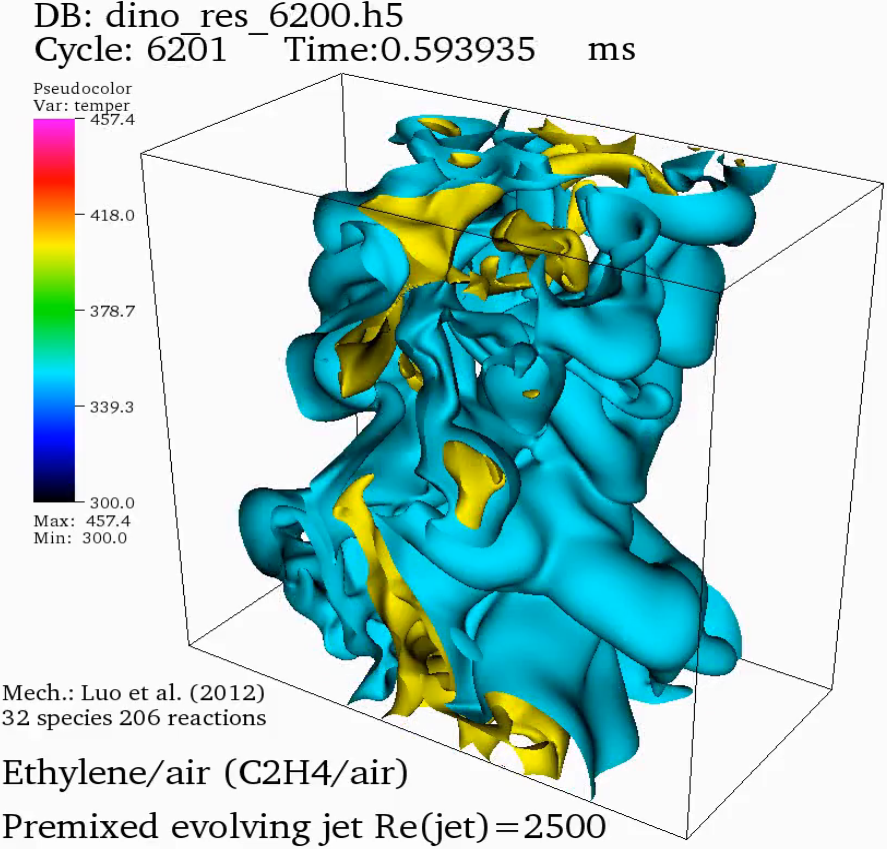
\includegraphics[width=0.8\textwidth]{figures/visit_isosurface.png}
    \caption{Temperature isosurfaces of a premixed jet flame.
        Simulated with DINO~\cite{Abdelsamie2016} and visualized using
        VisIt~\cite{HPV:VisIt}.}
    \label{fig:visit_isosurface}
\end{figure}
%
Combustion researchers have always used simple visualization methods to analyze
their data.
%
Plots of aggregated or point-wise variables over time, space, or other variables
give an idea about the state and behavior of the system.
%
Scatterplots reveal correlations and probability density functions that are the
basis for modeling turbulent combustion phenomena.
%

%
Every commercial and open source software package for scientific visualization
offers basic facilities to explore the three-dimensional structure of the data.
%
Color-mapping on cutting planes (slicing) and isosurface rendering are among
the most commonly used techniques for visualizing scalar and velocity data.
%
For example, the shape of the flame is represented by an isosurface of the
temperature or mixture fraction (see \cref{fig:visit_isosurface}).
%
Isosurfaces or slices of the velocity magnitude and vorticity are often used to
get a rough idea about the shape and turbulence level of the flow.
%
Scientists sometimes use direct volume rendering to show the full \ac{3D} data.
%
This is particularly attractive as it allows visualizing several variables at
the same time by carefully choosing transfer functions.
%
If the detailed structure of the flow field is important, it is often visualized
with streamlines, although this is less useful for high levels of turbulence.
%

%
Multiple simple techniques can be combined to build more powerful visualization
pipelines.
%
As an example, a combustion researcher might first extract the isosurface of
the stoichiometric mixture fraction as a representative of the flame front.
%
She then applies a temperature threshold to extract all regions of the flame
surface that are currently considered extinguished.
%
In these regions, she plots a histogram of the instantaneous strain rate of the
surface and compares it with a histogram of the same variable for the burning
regions of the flame, to investigate the statistical significance of the strain
rate for local extinction.
%

%
As the size of the raw data increases, visualization often has to be performed
on a supercomputer as well.
%
Many supercomputing centers have clusters with dedicated visualization nodes or
entirely separate clusters for visualization.
%
Visualization software such as ParaView~\cite{Ahrens2005} and
VisIt~\cite{HPV:VisIt} have the capability to run on supercomputing clusters
and split the work of processing and rendering datasets over many processes.
%
% subsubsection basic_visualization (end)
%
\subsubsection{Special Methods for Turbulent Combustion} % (fold)
\label{ssub:special_methods_for_turbulent_combustion}
%
Basic visualization techniques can go a long way towards assisting researchers
in analyzing their simulation data.
%
However, specialized methods are sometimes needed if the research question is
very complex or the computational demands are high.
%
Here we discuss some visualization and analysis tools that were developed
specifically for turbulent combustion applications.
%

%
Zistl \etal{}~\cite{Zistl2009} developed a toolbox focused on the analysis of
\ac{DNS} data.
%
It combines steps such as geometrical analysis of the flame surface and flame
structure, quantification of turbulent flow properties and turbulence/flame
interaction, and statistical analysis.
%
This allows for a more streamlined process when performing common research
tasks on the data.
%

%
Another group of visualization tools focus on the identification and tracking of
volumetric features.
%
Bremer \etal{} precompute a merge-tree representation and an accompanying
segmentation of volumetric \cite{Bremer2009,Bremer2011} and surface features
\cite{Bremer2010} defined by thresholding.
%
This allows an interactive post-hoc exploration of the threshold parameter
space and resulting tracking graph representing the evolution of features over
time.
%
Wang \etal{}~\cite{Wang2013} focuses on an efficient parallel algorithm to
identify and track volumetric features in a distributed memory environment
where features may span several processors.
%
Schnorr \etal{}~\cite{Schnorr2018} track cells in a space-filling topological
segmentation defined by the Morse-Smale decomposition of a scalar variable (see
\cref{sub:scalar_geometry_based}) by solving two graph optimization problems.
%
These cells, which are called dissipation elements in combustion literature,
carry significance in flamelet modeling.
%

%
As a first step towards analyzing unsteady features, some \ac{DNS} codes have
begun saving large amounts of Lagrangian particles (pathlines) and the
accompanying time series of simulation variables in addition to snapshots of the
(Eulerian) state of the simulation.
%
These pathlines allow the tracking of volumetric features even in snapshots with
large temporal gaps, as shown by Sauer \etal{}~\cite{Sauer2014}.
%
They can also be visualized by themselves, to get an idea about the dynamic
behavior of the system.
%
Wei \etal{}~\cite{Wei2011} developed a technique that combines a visualization
of particles in physical space with a visualization in the temperature --
mixture fraction phase space.
%
Trajectories are clustered in phase space to identify different chemical
behaviors, and the classes are then displayed in physical space for a visual
analysis (see \cref{fig:wei_particle_clusters}).
%
\begin{figure}[t]
    \centering
    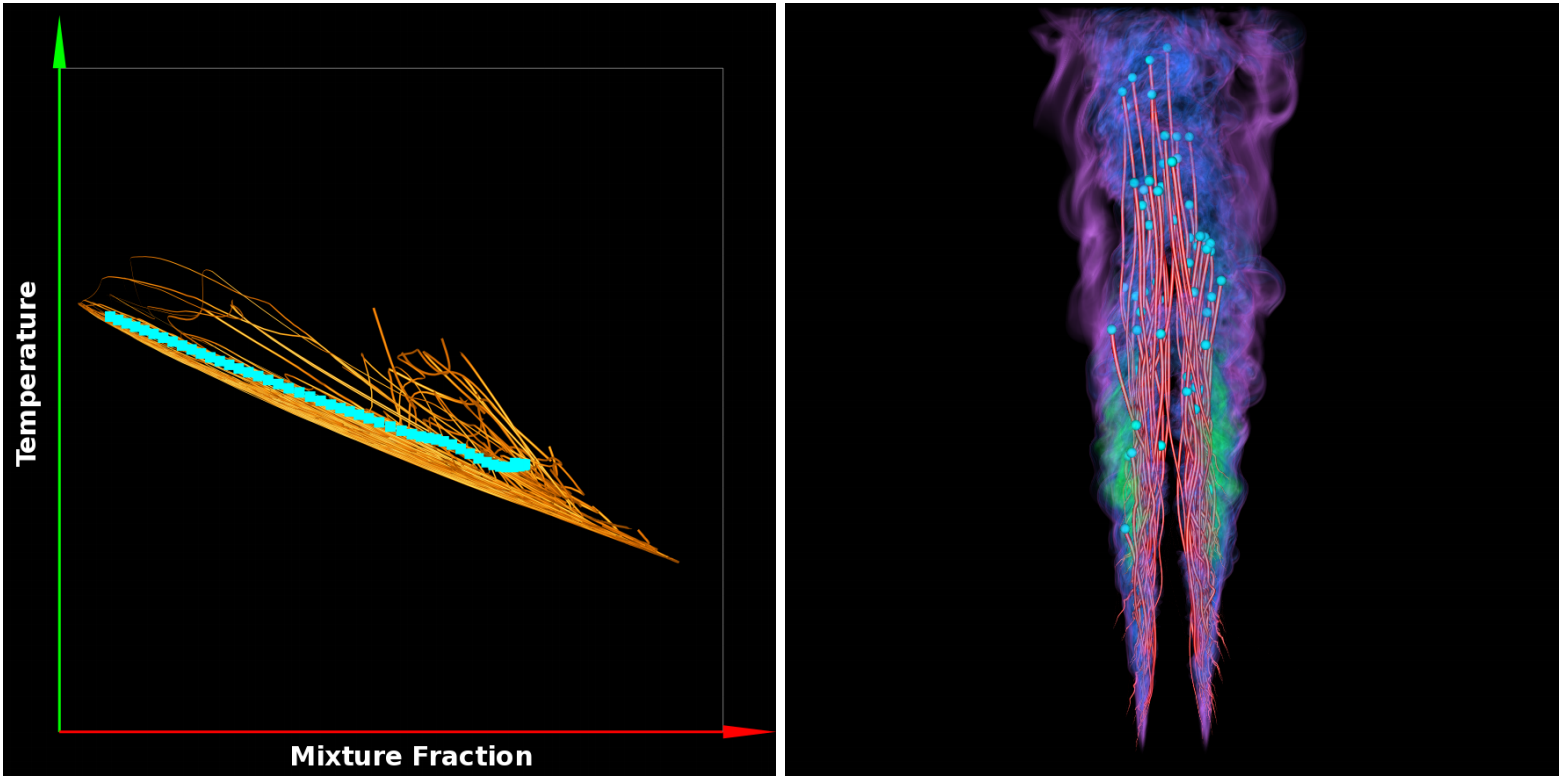
\includegraphics[width=\textwidth]{figures/wei_particle_clusters.png}
    \caption{Hybrid visualization of particle trajectories in phase space (left)
    and physical space (right) of an ethylene/air jet flame. Image source:
    Wei \etal{}~\cite{Wei2011}.}
    \label{fig:wei_particle_clusters}
\end{figure}
%
% subsubsection special_methods_for_turbulent_combustion (end)
%
% subsection post_processing (end)
%
\subsection{In-Situ Processing} % (fold)
\label{sub:in_situ_processing}
%
With disk space and I/O speed being the bottleneck in today's large-scale
simulations, in-situ approaches to visualization and analysis have gained
popularity through the last 15 years.
%
Here, the visualization and analysis of the data is performed in parallel or
interleaved with the simulation, without first writing it to a hard disk.
%
This allows for the analysis of the complete simulation output, rather than
the infrequent snapshots that are used in post-processing approaches.
%
Ma gave an overview of the problems and opportunities inherent in in-situ
visualization~\cite{Ma2009}.
%

%
A central complication of in-situ approaches is the loss of flexibility and
interactivity.
%
Large simulations typically need to be submitted to a job queue before they are
started on a supercomputing cluster.
%
This means that there might be a significant waiting time before any results can
be viewed.
%
It is often unreasonable to expect that an analyst is present to look at the
data while some interesting feature or behavior can be observed during the
simulation.
%
Additionally, simulations can take several days or even weeks to complete.
%
This makes an exploratory analysis of the data very challenging.
%
Many in-situ approaches therefore have a batch processing character, where
visualization and analysis tasks are defined beforehand and are then
carried out during the simulation with little to no user input.
%
The user then explores the significantly smaller results, which ideally still
contain all relevant information.
%

%
Another problem is performance.
%
Since large simulations can already take a very long time, researchers are
reluctant to accept a significant increase in computing time in return for
visualization.
%
The simulation data is distributed across the nodes of the supercomputer to
optimize the simulation time.
%
This is not necessarily an optimal distribution for visualization tasks.
%
The result can be a significant communication overhead, which is a major
bottleneck in supercomputing clusters.
%
In-situ algorithms need to be carefully crafted to find a good balance between
communication overhead and efficiency gained by data reorganization.
%

%
A lot of groundwork is being done to create the foundations for successful
in-situ processing.
%
We will first give an overview of these technical contributions and then present
some examples for specific in-situ visualization techniques.
%
\subsubsection{Technical Foundations} % (fold)
\label{ssub:technical_foundations}
%
In-situ processing is a complex task not only from a conceptual, but also from a
software engineering perspective.
%
In-situ algorithms need to run on large supercomputers in parallel or even on
the same nodes as the simulations.
%
They need to somehow get the relevant data from the simulation and they need to
be efficient enough to not slow it down by an unreasonable amount.
%
Communication between computing nodes flows over relatively slow network
connections, requiring different parallel algorithms than for shared-memory
multi-core architectures.
%
Additionally, computing nodes often do not have dedicated graphics hardware,
which makes software rendering a necessity.
%
All this requires a solid technical foundation of systems and algorithms that
facilitate the visualization and analysis tasks that eventually derive insight
from simulations.
%

%
The two most popular open source software packages for scientific visualization,
ParaView and VisIt, both include an extension for in-situ visualization.
%
In the case of ParaView, it is called Catalyst~\cite{Ayachit2015}.
%
VisIt's in-situ library is LibSim~\cite{Whitlock2011}.
%
Both require a certain amount of instrumentation of the simulation code to
function.
%
If a simulation code has been interfaced with the visualization software, it
communicates its data to parallel visualization server processes that are
launched together with the simulation and eventually to a client that
allows a similar interaction as if the data was loaded from a file.
%
In addition, the user can define non-interactive batch visualization tasks that
are executed regularly and produce images or data files.
%

%
Larsen \etal{} presented a simpler and more flexible system that only supports
batch visualization with Strawman~\cite{Larsen2015}.
%
It is based on EAVL~\cite{Meredith2012}, a visualization library that is
designed fundamentally to run on massively parallel architectures.
%
Libraries with similar goals exist in DAX~\cite{Moreland2011} and
PISTON~\cite{Lo2012}.
%
All three have merged their efforts into a single project:
VTK-m~\cite{Moreland2016}.
%
The goal is to develop a native visualization library for supercomputers and
other highly parallel architectures that can be a basis for scientific
visualization in a future with steadily growing data sizes and a growing need
for in-situ capabilities.
%

%
Many existing tools for in-situ processing require changes to the simulation
code in order to receive data from it.
%
This can be an additional obstacle for the adaption of these tools by simulation
scientists.
%
One possibility to reduce this invasiveness is to link the visualization and
analysis tasks to the I/O library the simulation code uses to write out its
data~\cite{Vishwanath2011,Biddiscombe2011,Dorier2013}.
%
This unifies the tasks of writing snapshots to disk, analyzing and visualizing
them into the same framework and effectively decouples them from the simulation
itself.
%
The Freeprocessing system~\cite{Fogal2014} takes an even less invasive approach.
%
It places itself between the I/O calls and the simulation code at library load
time, requiring no changes to the simulation code at all.
%

%
Another focus of research has been dedicated to improving performance.
%
Researchers have tried sophisticated load-balancing algorithms to take advantage
of unused resources during a simulation run for visualization and analysis tasks
\cite{Zheng2013}.
%
A popular alternative to processing the data on the same computing nodes as the
simulation is to offload it onto a separately allocated number of staging or
processing nodes
\cite{Zheng2010,Abbasi2010,Abbasi2011,Docan2011,Docan2012,Bennett2012}.
%
Using this approach, which is often called \emph{in-transit} processing, the
simulation is only slowed down by the time it takes to copy the data to the
staging nodes, where processing can happen in parallel to the next simulation
step.
%
Some work has also been done to optimize existing parallel rendering algorithms
for use on supercomputing
clusters \cite{Yu2008,Kendall2010,Moreland2011a,Cavin2012,Nonaka2014,Grosset2016}.
%

%
In all of the works presented above, efficiency and convenience of in-situ
processing was the focus.
%
The second major problem, namely the lack on interactivity, has been addressed
to a lesser extent.
%
Maybe that is because it is much harder to solve.
%
The challenge is to enable an exploratory analysis of the simulation data,
\ie{}, with little to no prior knowledge of what one is looking for.
%
This stands in direct conflict with the goal of in-situ approaches to reduce the
amount of data that has to be stored to disk.
%
In order to reduce the data, one must know what is or is not important.
%
A small number of works has tried to address this issue.
%

%
One obvious possibility is to compress the data using some generic concept of
``importance'' that is not dependent on a particular application.
%
Lakshminarasimhan \etal{}~\cite{Lakshminarasimhan2011} developed such an
algorithm whose core idea is to sort the data before compression to take
advantage of the special characteristics of scientific data.
%
With a compression ratio of about 1:7, this approach allows to store a much
larger amount of data while still retaining complete freedom for an exploratory
analysis of the data.
%

%
Another approach has been proposed by Kageyama and Yamada~\cite{Kageyama2014}
and Ahrens \etal{}~\cite{Ahrens2014}:
%
Produce a database of visualizations that the user can explore later.
%
During the simulation, rendered images are produced for a range of parameters
of the same visualization.
%
For example, isosurfaces of different variables with different iso-levels are
rendered from different camera angles and stored into the database.
%
The user can then select a set of parameters after the fact, retrieve the
best fitting image from the database, and even compose multiple images into
a combined visualization.
%

%
All these contributions address different issues that need to be solved for
in-situ processing to become successful.
%
Since the field is still in its infancy, no clear favorites have emerged yet and
a definitive in-situ framework has yet to be developed.
%
% subsubsection technical_foundations (end)
%
\subsubsection{Special Visualization and Analysis Methods} % (fold)
\label{ssub:visualization_and_analysis_methods}
%
Although most work in the field of in-situ visualization has been done to lay
the groundwork for efficient basic visualization, there have been some
developments of more specialized in-situ methods.
%
We will discuss some examples here that are applicable to the field of turbulent
combustion.
%

%
The first in-situ visualization methods focused on rendering images for
monitoring the simulation.
%
Yu \etal{}~\cite{Yu2010} used their parallel direct volume rendering and image
compositing algorithm \cite{Yu2008} to display scalar variables in combustion
simulations together with particles advected with the flow.
%
This gives an idea about the evolution of the simulation but does not allow for
quantitative analysis of the data.
%
Tikhonova \etal{}~\cite{Tikhonova2011} developed a more flexible approach by
rendering the data into an intermediate representation that stores an
attenuation function instead of color values.
%
The transfer function can then be changed after the fact, allowing for a certain
degree of interactivity (see \cref{fig:tikhonova_tf}).
%
This approach fits well with the image databases discussed in the previous
section \cite{Kageyama2014,Ahrens2014}.
%
\begin{figure}[t]
    \begin{captionbeside}{
        Retroactive adjustment of the transfer function in direct volume
        renderings of a turbulent jet flame. Left: original transfer function.
        Middle: Opacity modulation. Right: Opacity modulation and
        re-colorization. Image source: Tikhonova \etal{}~\cite{Tikhonova2011}.
        \label{fig:tikhonova_tf}
    }[o]
        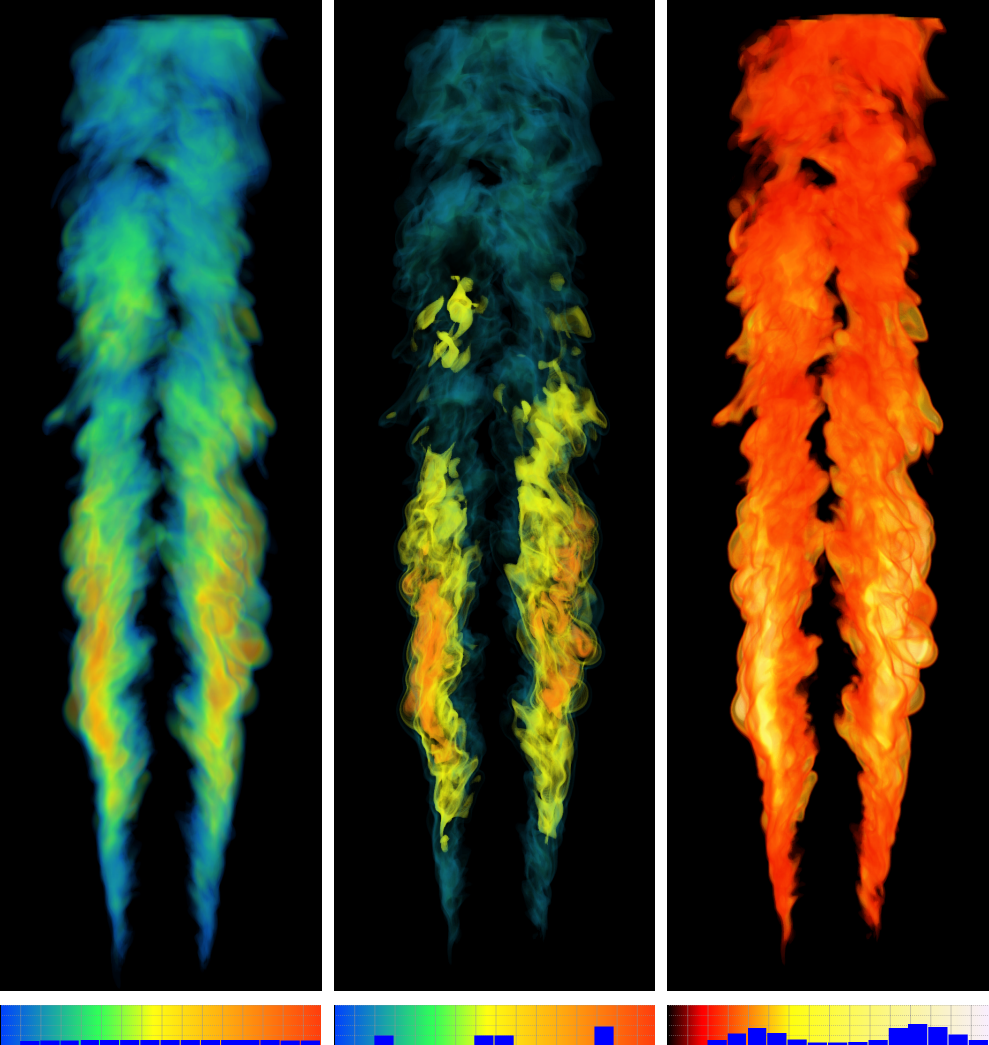
\includegraphics[width=0.6\textwidth]{figures/tikhonova_transfer_function.png}
    \end{captionbeside}
\end{figure}
%

%
Moving on to more analytic approaches, several works have addressed the
extraction and tracking of volumetric features.
%
Chen \etal{}~\cite{Chen2003} presented an in-situ system for tracking volumetric
features defined by thresholding.
%
Zhang \etal{}~\cite{Zhang2012} used the \ac{DOC} algorithm \cite{Quiroz2008} to
identify and track features defined by clusters in state space during a
simulation run.
%
This can for example be used to identify and track burning regions in combustion
simulations.
%
The IFDT framework \cite{Duque2012} takes a more flexible approach by letting a
user interactively pick individual structures to track.
%
The system includes a machine learning component that learns to identify the
features picked by the user based on their visual properties.
%
This is intended to be more robust than detection based on thresholds which
might not be applicable over long time periods.
%
Ye \etal{}~\cite{Ye2015} combined image-based visualization with feature
tracking by storing rendered depth maps of multiple isosurfaces.
%
These are later used to create visualizations and to track features in image
space based on their depth information.
%
\Cref{cha:flame_surface_tracking} of this thesis presents an in-situ tracking
algorithm for surfaces which explicitly captures temporal correspondence and
tangential movement of surface points.
%

%
The idea of precomputing an intermediate representation of the data in-situ and
then exploring it post-hoc has also been applied in some more specialized
visualization systems.
%
Landge \etal{}~\cite{Landge2014} adapted the computation of segmented merge
trees \cite{Bremer2009,Bremer2011} for in-situ applications.
%
This allows for an interactive exploration of the space of possible thresholds
or iso-levels for scalar variables.
%
Ye \etal{}~\cite{Ye2016} proposed a system for exploring joint field/particle
datasets as are for example produced by some combustion \ac{DNS} codes.
%
They compute \acp{PDF} to represent the field data, and reorganize the particle
data into a more efficient scheme.
%
Researchers can then explore the \acp{PDF} in a post-hoc tool and define queries
to select matching particle data.
%
A space-saving representation for post-hoc analysis of premixed combustion data
is presented in \cref{cha:sparse_representation} of this thesis, although not as
an in-situ algorithm.
%
%
% subsubsection visualization_and_analysis_methods (end)
%
% subsection in_situ_approaches (end)
%
% section visualization_for_turbulent_combustion_simulations (end)